\subsection{Messungen}
In diesem Abschnitt sollen charakteristische Messwerte der Fahrspurerkennung, Regelung, sowie dem Zusammenspiel beider Komponenten dargestellt und diskutiert werden. Dies soll unter Veränderung der Umgebungsbedingungen sowie mit unterschiedlichen Fortbewegungsgeschwindigkeiten des Modellfahrzeugs geschehen.
  
\subsubsection{Evaluation ohne Ground Truth}
Für die Erkennung von Fahrspuren auf Einzelbildern und die daraus resultierende Bewegung des Fahrzeugs existieren zum jetzigen Zeitpunkt keine Vergleichswerte. 

\paragraph{Bildverarbeitung} 
Für ein Benchmark der Fahrspurerkennung könnte ein Ground-Truth-Datensatz in Form von Bildern mit richtig eingetragen Fahrbahnmarkierungen die präziseste Bewertung hervorbringen. Da die Erstellung eines solchen jedoch sehr zeitaufwendig ist, wurde eine leichter automatisierbare Methode der Evaluation gewählt.

Durch die implementierte Verifikation der erkannten Koordinatenserien kann eine Fehlerkennung weitgehend ausgeschlossen werden. Den deutlichsten Indikator für ein falsch verarbeitetes Bild stellt also eine nicht oder nur auf einem sehr kurzen Abschnitt detektierte Fahrbahnmarkierung dar. Den Grenzwert der Länge für eine fehlerhaft erkannte Linie ist oft unkritisch, da der Detektionsalgorithmus in den meisten Fällen zufriedenstellend funktioniert oder schon bei kurzer Linienlänge fehlschlägt. Wir haben uns dafür entschieden etwa die halbe Sichtweite des Fahrzeugs (ab Stoßstange bis Bildrand ) als Schwellwert anzusehen.

\paragraph{Regelung} 
Die Güte der Regelung bzw. des Zusammenspiels aus Bildverarbeitung und Regelung könnte am exaktesten durch ein hinreichend genaues System zur Lokalisierung des Fahrzeugs im Testszenario ermittelt werden. Somit wäre es möglich die Abweichung der gefahrenen Strecke von einer vorgegebenen Ideallinie auszuwerten. Da die Inbetriebnahme des an der Professur vorhandenen zweidimensionalen Tracking-Systems viel Einarbeitungszeit benötigt, wird hier auf eine einfache Methode zurückgegriffen. Es wird lediglich vermerkt ob das Fahrzeug die Fahrspur völlig verlässt oder dem Straßenverlauf zufriedenstellend folgt.

\subsubsection{Parametertuning}
Dieser Paragraph beschäftigt sich mit der Ermittlung der maximal fahrbaren Geschwindigkeit bei Nutzung der entwickelten Bildverarbeitungs- und Regelungsstruktur. Durch die Auswertung verschiedener Messwerte soll der \glqq Flaschenhals\grqq\ gefunden und, wenn möglich, durch Parameteranpassung beseitigt werden.

Wichtige, noch anzupassende Parameter stellen dar:
\begin{itemize}
\item Die Frequenz, in der Bilder verarbeitet werden
\item Die Frequenz, mit der die Regelung stattfindet
\item Die Entfernung des Zielpunktes der Regelung vom Fahrzeug
\end{itemize}

Den Ausganspunkt für die folgenden Optimierungen bildet eine Geschwindigkeit von
\SI{0.1}{\metre\per\second}. Die Frequenz, mit welcher die Bilder verarbeitet werden wurde auf \SI{1}{\hertz} festgelegt, da die Extraktion der Linienpunkte eines Testbildes ca. \SI{0.5}{\second} benötigt. Die Frequenz der Regelung wurde initial auf \SI{20}{\hertz} festgelegt, da der Rechenaufwand für einen Regelungszyklus sehr gering ist. Eine noch höhere Regelfrequenz verspricht keinen Performancegewinn und läge schon nahe der maximalen Ansteuerfrequenz des Lenkservos sowie der Abtastrate der \gls{acr:imu} (jeweils \SI{50}{\hertz}).

Mithilfe dieser Einstellung absolvierte das Fahrzeug erfolgreich eine Runde im Testparcours. Wie in Abb.~\ref{fig:evaluation:riverflow:times_combined_1Hz_0_1m_s_over_piciter} zu sehen, benötigt ein Bild-Callback im Echtzeitbetrieb, d.h. bei mehrmaliger Ausführung erheblich weniger Zeit als beim einmaligen Messung anhand eines Testbildes. Die Verringerung der Bearbeitungsdauer \scl{t_{img}} von ca. \SI{500}{\milli\second} auf \SI{128}{\milli\second} (Median der in Abb.~\ref{fig:evaluation:riverflow:times_combined_1Hz_0_1m_s_over_piciter} dargestellten Daten) lässt sich unter anderem durch die Fahigkeit MATLABs, Funktionen bei wiederholter Ausführung im Hauptspeicher zu halten und somit schneller ausführen zu können, erklären. Eine signifikante Erhöhung der Bildfrequenz \scl{f_{img}} ist also möglich. Nimmt man die vom der Regelung und Posenaktualisierung, d.h. dem Odometrie-Callback  pro Sekunde benötigte Zeit \scl{t_{odom-per-sec}} als konstant an, lässt sich die theoretisch mögliche Bildfrequenz wie folgt berechnen:
\begin{subequations}
\begin{equation}
	T_{img} = t_{img}+t_{odom-per-sec}\cdot T_{img}
\end{equation}
%\begin{equation}
%	T_{img}\cdot(1-t_{odom-per-sec}) = t_{img}
%\end{equation}
\begin{equation}
	T_{img} = \frac{t_{img}}{1-t_{odom-per-sec}}
\end{equation}
\begin{equation}	
	f_{img} = \frac{1}{T_{img}}
\end{equation}
\end{subequations} 
Mit einer Bildbearbeitungszeit \(t_{img}=\SI{128}{\milli\second}\) sowie dem Zeitbedarf des Odometrie-Callbacks von \(t_{odom-per-sec}=\SI{262}{\milli\second\per\second}\) ergibt sich eine in der Theorie nutzbare Framerate von über \SI{5}{\hertz}. Mit dieser Bildfrequenz wurde eine weitere Testfahrt absolviert, in Abb. \ref{fig:evaluation:riverflow:times_pic_5Hz_0_2m_s_over_piciter} wird die bessere Nutzung der zur Verfügung stehenden Rechenzeit deutlich. Abbildung \ref{fig:evaluation:riverflow:times_pic_5Hz_0_2m_s_over_piciter} zeigt jedoch, dass die Periodendauer der Bildverarbeitung zwischen 2 Punkten oszilliert. Der erwartete zeitliche Abstand zweier konsekutiver Aufnahmen von \SI{200}{ms} wird häufig nicht erreicht, stattdessen befindet sich ein Abstand von \(2 \cdot \SI{200}{ms} = \SI{400}{ms}\) zwischen aufeinander folgenden Bildern. Dies führt zu dem Schluss, dass durch nicht vorhandene Pufferung Aufnahmen ausgelassen wurden.

\begin{figure}[ht] % [htb]
\centering
\subfloat[\SI{5}{\hertz}\label{fig:evaluation:riverflow:times_pic_5Hz_0_2m_s_over_piciter}]{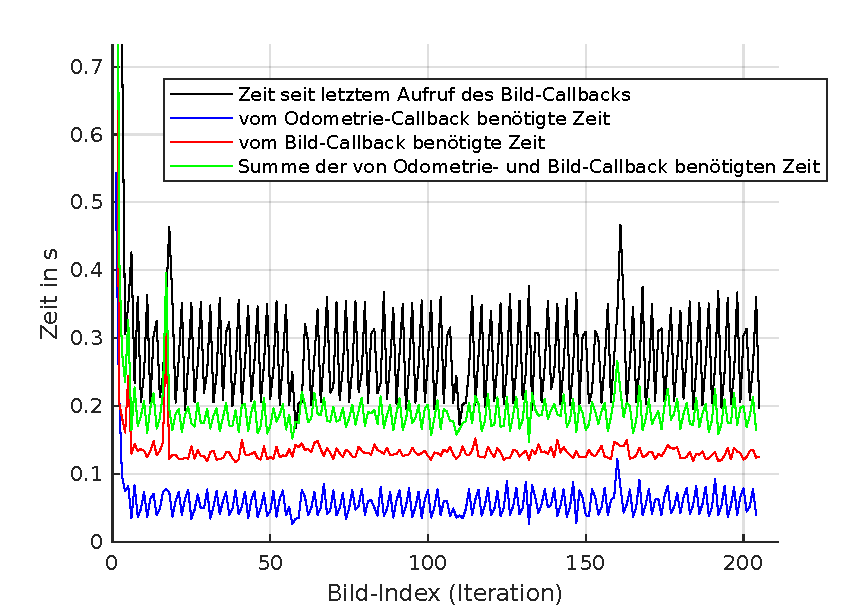
\includegraphics[width=0.45\textwidth]{evaluation_riverflow_times_combined_5Hz_0_2m_s_over_piciter}}
\qquad
\subfloat[\SI{4}{\hertz}\label{fig:evaluation:riverflow:times_pic_4Hz_0_2m_s_over_piciter}]{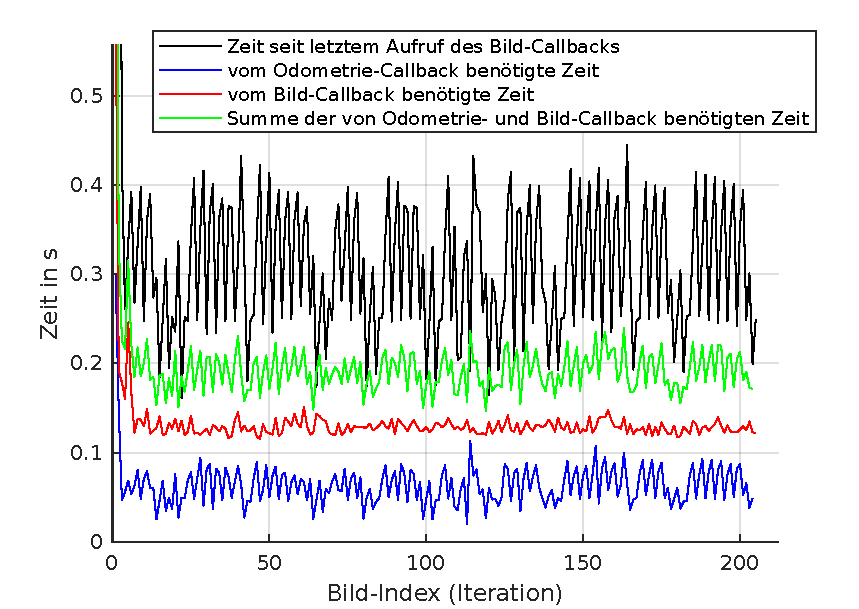
\includegraphics[width=0.45\textwidth]{evaluation_riverflow_times_combined_4Hz_0_2m_s_over_piciter}}
\qquad
\subfloat[\SI{3}{\hertz}\label{fig:evaluation:riverflow:times_pic_3Hz_0_2m_s_over_piciter}]{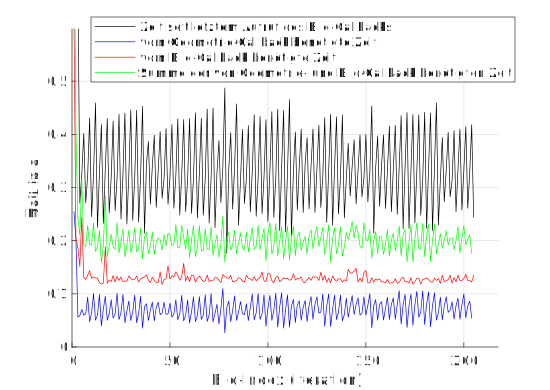
\includegraphics[width=0.45\textwidth]{evaluation_riverflow_times_combined_3Hz_0_2m_s_over_piciter}}
\subfloat[\SI{1}{\hertz}\label{fig:evaluation:riverflow:times_combined_1Hz_0_1m_s_over_piciter}]{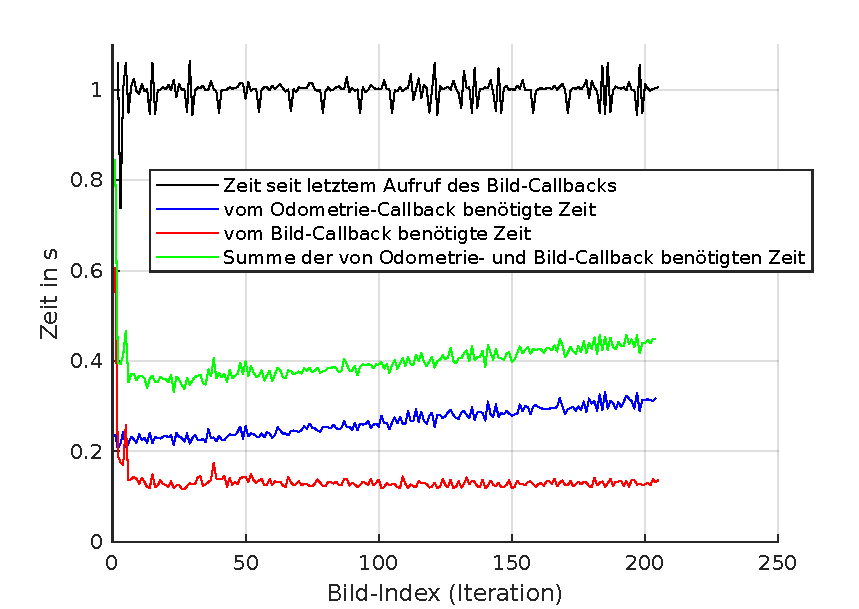
\includegraphics[width=0.45\textwidth]{evaluation_riverflow_times_combined_1Hz_0_1m_s_over_piciter}}
\caption{Zeitbedarf aller Fahrspurverfolgungskomponenten bei \SIlist{5;4;3;1}{\hertz} Bildfrequenz}
\end{figure}

Im folgenden wurde die Bildfrequenz zuerst auf 4 (s.Abb. \ref{fig:evaluation:riverflow:times_pic_4Hz_0_2m_s_over_piciter}), später auf \SI{3}{\hertz} verringert (s.Abb. \ref{fig:evaluation:riverflow:times_pic_3Hz_0_2m_s_over_piciter}). Erst jetzt konnte kein Springen der Periodendauer des Bild-Callbacks auf ein Vielfaches seines Erwartungswertes mehr festgestellt werden. Eine leichte Oszillation des zeitlichen Abstands zweier Aufnahmen ist auch in Abb. \ref{fig:evaluation:riverflow:times_pic_3Hz_0_2m_s_over_piciter} zu erkennen, jedoch beträgt der Mittelwert fast exakt die erwarteten \SI{333}{ms}. Die verbleibenden Unregelmäßigkeiten sind auf den Kamera-Node, welcher die Bilder aufnimmt und im entsprechenden Topic veröffentlicht, hervorgerufen werden (s. Abschnitt \ref{ssec:software_struktur:ros:nodes}). Abbildung \ref{fig:evaluation:riverflow:times_combined_3Hz_0_2m_s_pie_median} bzw. \ref{fig:evaluation:riverflow:times_combined_3Hz_0_2m_s_pie_mean} stellt nocheinmal die pro Bild mit Regelung,Bildverarbeitung,sonstigem Overhead\& im Leerlauf verbrachte Zeit einer gefahrenen Runde dar.

\begin{figure}[ht] % [htb]
	\centering
	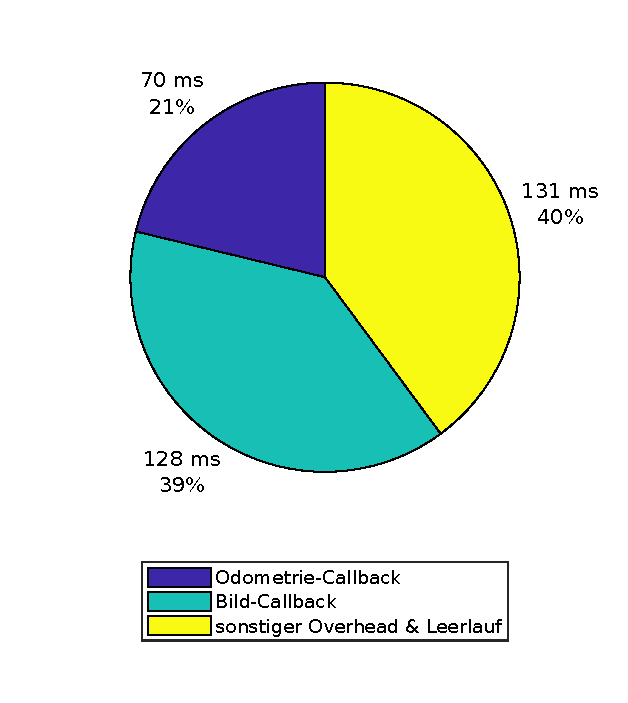
\includegraphics[width=0.7\textwidth]{evaluation_riverflow_times_combined_3Hz_0_2m_s_pie_median}
	\label{fig:evaluation:riverflow:times_combined_3Hz_0_2m_s_pie_median}
	\caption{Zeitbedarf aller Fahrspurverfolgungskomponenten bei \SI{3}{\hertz} Bildfrequenz; Median aller Messwerte einer Runde der Teststrecke}
\end{figure}

\begin{figure}[ht] % [htb]
	\centering
	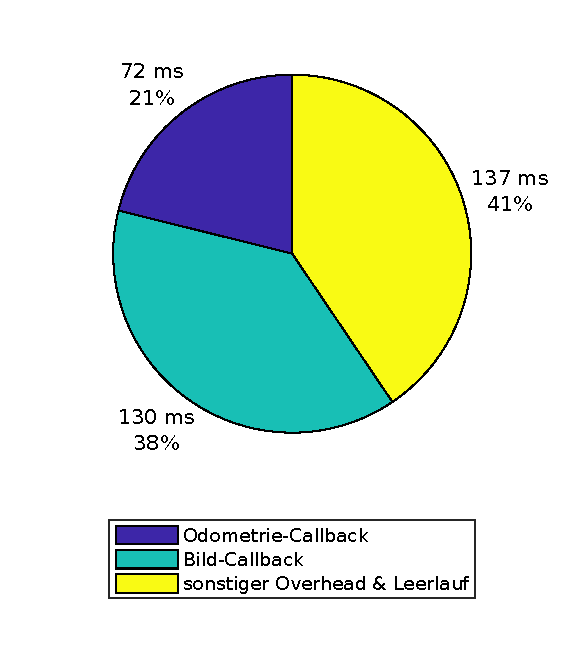
\includegraphics[width=0.7\textwidth]{evaluation_riverflow_times_combined_3Hz_0_2m_s_pie_mean}
	\label{fig:evaluation:riverflow:times_combined_3Hz_0_2m_s_pie_mean}
	\caption{Zeitbedarf aller Fahrspurverfolgungskomponenten bei \SI{3}{\hertz} Bildfrequenz; Mittelwert aller Messwerte einer Runde der Teststrecke}
\end{figure}

\paragraph{Dauer einzelner Komponenten der Fahrspurerkennung}
Um in Zukunft Optimierungen an den implementierten Bildverarbeitungsalgorithmen durchführen zu können ist es unumgänglich nicht nur die gesamt benötigte Zeit, sondern auch die Dauer der einzelnen Module zu messen.

\begin{figure}[ht] % [htb]
	\centering
	\subfloat[Boxplot ohne Startphase\label{fig:evaluation:riverflow:times_pic_3Hz_0_2m_s_boxplot}]{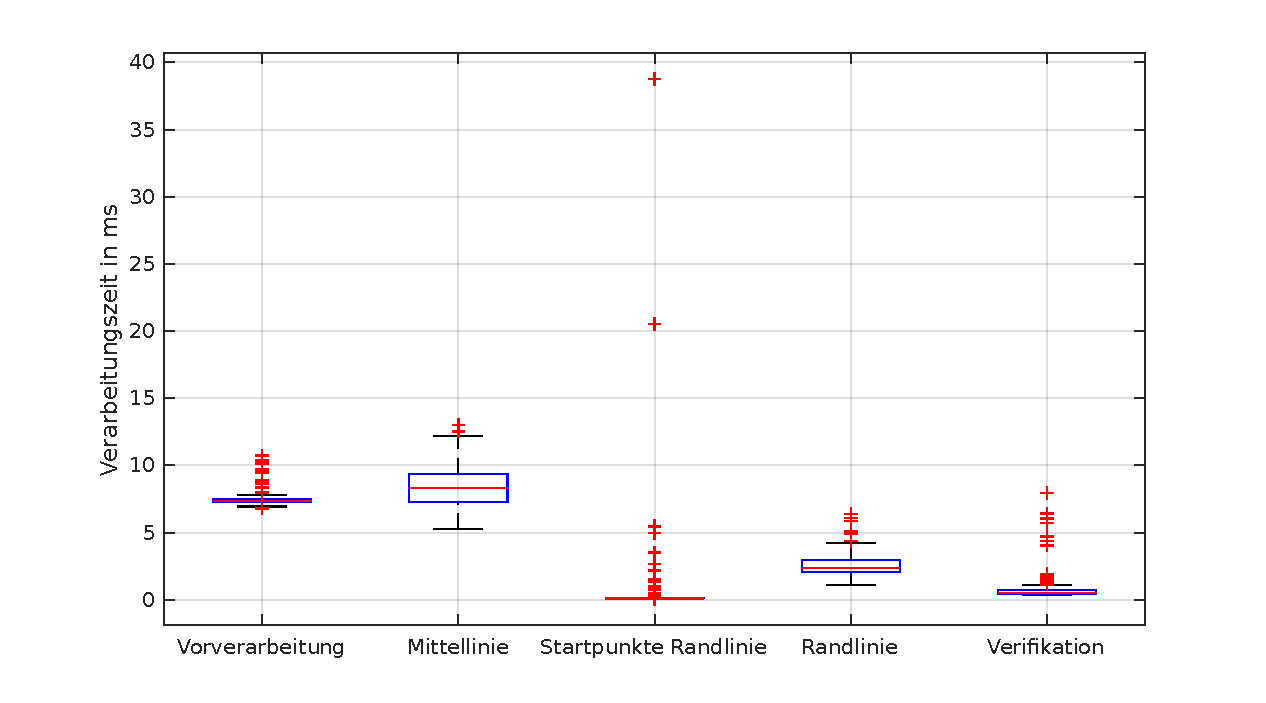
\includegraphics[width=0.7\textwidth]{evaluation_riverflow_times_pic_3Hz_0_2m_s_boxplot}}
	\qquad
	\subfloat[Boxplot ohne Startphase\label{fig:evaluation:riverflow:times_pic_3Hz_0_2m_s_boxplot_ros}]{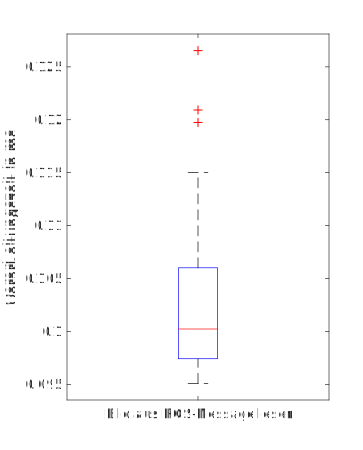
\includegraphics[width=0.2\textwidth]{evaluation_riverflow_times_pic_3Hz_0_2m_s_boxplot_ros}}
	\subfloat[Tortendiagramm; Median aller Messwerte einer Runde\label{fig:evaluation:riverflow:times_pic_3Hz_0_2m_s_pie_no_ros}]{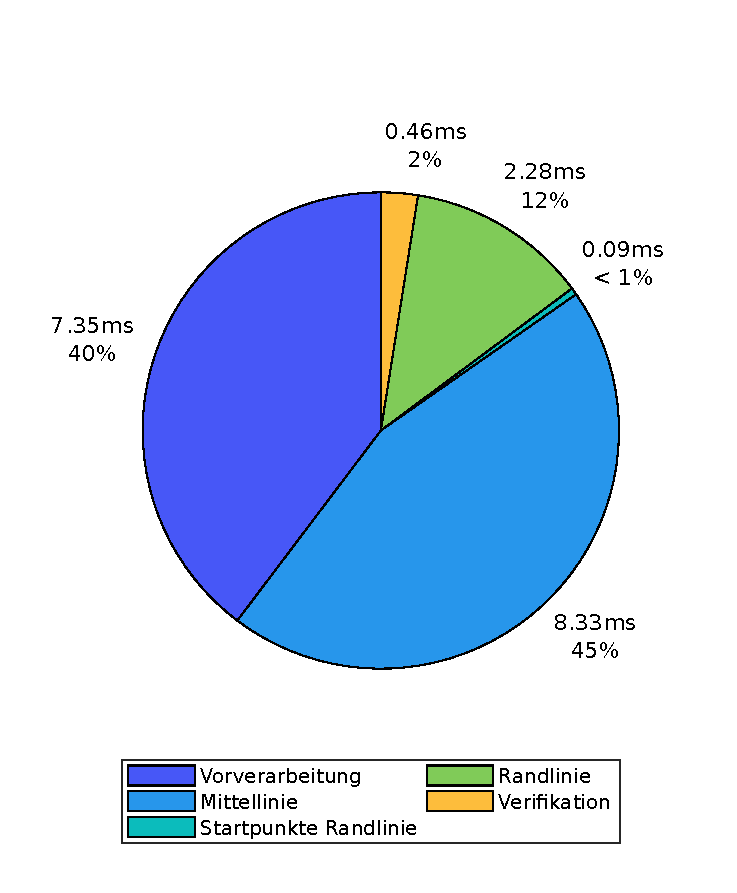
\includegraphics[width=0.45\textwidth]{evaluation_riverflow_times_pic_3Hz_0_2m_s_pie_no_ros}}
	%Summe:18.5185ms
	\qquad
	\subfloat[Tortendiagramm; Median aller Messwerte einer Runde; mit Dekompression des Bildes\label{fig:evaluation:riverflow:times_pic_3Hz_0_2m_s_pie_with_ros}]{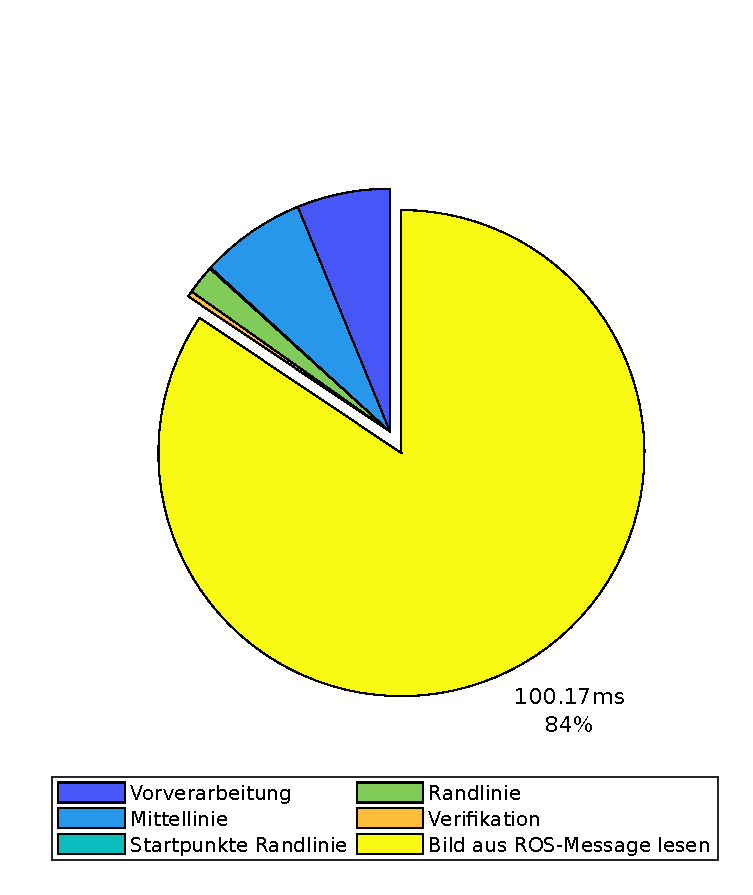
\includegraphics[width=0.45\textwidth]{evaluation_riverflow_times_pic_3Hz_0_2m_s_pie_with_ros}}
	\caption{Zeitbedarf aller Fahrspurerkennungskomponenten bei \SI{3}{\hertz} Bildfrequenz}
\end{figure}

Diese Untersuchungen führten zu interessanten Ergebnissen, welche die Echtzeitfähigkeit der MATLAB-\gls{acr:ros}-Schnittstelle in Frage stellen. Wie in Abbildung \ref{fig:evaluation:riverflow:times_pic_3Hz_0_2m_s_pie_with_ros} zu sehen, wird ein Großteil der Dauer eines Bild-Callbacks zum Umwandeln der \gls{acr:ros}-Message in eine von MATLAB prozessierbare Matrix benötigt. Eine genauere Untersuchung mit dem MATLAB-Profiler zeigte, dass in diesem Schritt eine Dekompression des im JPEG-Format übertragenen Bildes den wesentlichen Anteil dieses Zeitbedarfs verursacht. Eine unkomprimierte Übertragung würde jedoch ein vielfaches dieser Dauer in Anspruch nehmen.

Der eigens entwickelte Anteil der Fahrspurerkennung benötigt im Median einer Runde lediglich \SI{18,5}{ms}, die genaue Aufteilung kann in Abb. \ref{fig:evaluation:riverflow:times_pic_3Hz_0_2m_s_pie_no_ros} sowie \ref{fig:evaluation:riverflow:times_pic_3Hz_0_2m_s_boxplot} nachvollzogen werden. Die meiste Zeit wird für Bildvorverarbeitung und Mittellinienerkennung benötigt. Da diese Funktionen zum Großteil auf vorgegebenen, komplexen und bereits maschinennah implementierten MATLAB-Funktionen basieren, kann hier nur unter Nutzung anderer Software eine Optimierung stattfinden. Die zum Großteil aus elementaren Funktionen aufgebaute Erkennung\&Verifikation der Randlinie läuft schon erfreulich schnell ab, sodass hier trotz der vielen verwendeten, in MATLAB rechenzeitintensiven Schleifen keine zügigere Alternative gesucht werden muss.

\subparagraph{Startpunktfindung}
Wie in Abb. \ref{fig:evaluation:riverflow:times_pic_3Hz_0_2m_s_pie_no_ros} zu sehen, verstreicht im Normalfall bei der Feststellung der Startpunkte zur Erkennung der seitlichen Fahrbahnmarkierungen kaum Zeit. Wird jedoch kein Mittellinienelement nahe genug vor dem Fahrzeug gefunden, so gestaltet sich dieser Prozess aufwendiger (siehe Abschnitt \ref{sssec:fahrspurerkennung:riverflow:randlinie:startpunktgewinnung}). Abbildung \ref{fig:evaluation:riverflow:times_startpoints_3Hz_0_2m_s_boxplot} gibt ein besseres Bild der Messwerte wieder als Diagramm \ref{fig:evaluation:riverflow:times_pic_3Hz_0_2m_s_pie_no_ros} bzw. \ref{fig:evaluation:riverflow:times_pic_3Hz_0_2m_s_boxplot}, da hier nicht nur der Median aller Messwerte gebildet, sondern vor der Erstellung des Boxplots die Daten nach Art der Methode zur Startpunktbestimmung sortiert werden. 
\begin{figure}[ht] % [htb]
	\centering
	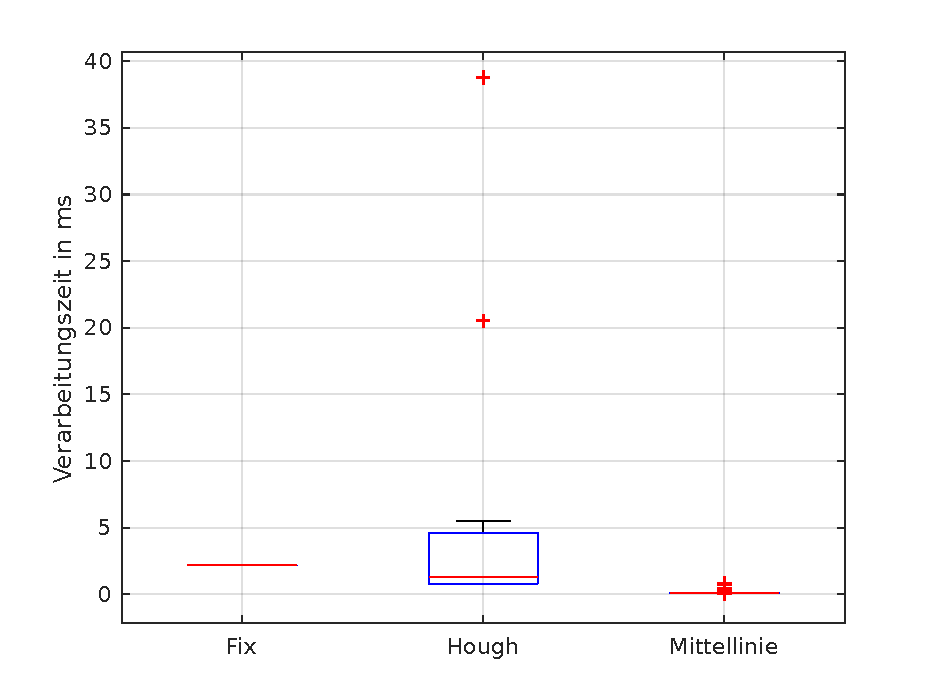
\includegraphics[width=0.7\textwidth]{evaluation_riverflow_times_startpoints_3Hz_0_2m_s_boxplot}
	\label{fig:evaluation:riverflow:times_startpoints_3Hz_0_2m_s_boxplot}
	\caption{Zeitbedarf der Startpunktfindungsalgorithmen für die Erkennung der seitlichen Fahrbahnmarkierungen bei \SI{3}{\hertz} Bildfrequenz}
\end{figure}
Die Erwartung, dass bei Nutzung der mittigen Fahrbahnmarkierung zu Startpunktgenerierung kaum Zeit vergeht, wurde durch den über diese Kategorie gebildeten Median von \SI{0,09}{ms} bestätigt. Jedoch ist auch die von der eindimensionalen Hough-Transformation benötigte Laufzeit von \SI{1,32}{ms} vertretbar. Die In Abbildung \ref{fig:evaluation:riverflow:times_startpoints_3Hz_0_2m_s_boxplot} sichtbaren Ausreißer entstehen durch das erstmalige ausführen der Funktion, welche nicht während der im Boxplot unberücksichtigten \glqq Warmlaufphase\grqq\ geschieht. Da nur einmal fix im Bildkoordinatensystem liegende Punkte genutzt werden mussten und dieser Fall nur nach Fehlschlag der eindimensionalen Hough-Transformation auftritt, wird dieser Messwert nur als Median ohne Box etc. in Abb. \ref{fig:evaluation:riverflow:times_startpoints_3Hz_0_2m_s_boxplot} dargestellt und bewegt sich mit \SI{2,17}{ms} im Bereich dieser Methode.

\paragraph{Übertragungszeit}
Die Übertragungszeit der Bilder von \SI{77,2}{ms} im Median stellt eine erhebliche Totzeit dar. Die Streuung dieser bis hin zu \SI{183}{ms} spiegelt die Probleme der Nutzung einer WLAN-Verbindung, welche gern zu unvorhersehbaren Latenzen neigt, wieder. Durch eine JPEG-Kompression mit einer Qualitätseinstellung von 20\% wurde der Bildtransfer schon signifikant beschleunigt.

\begin{figure}[ht] % [htb]
	\centering
	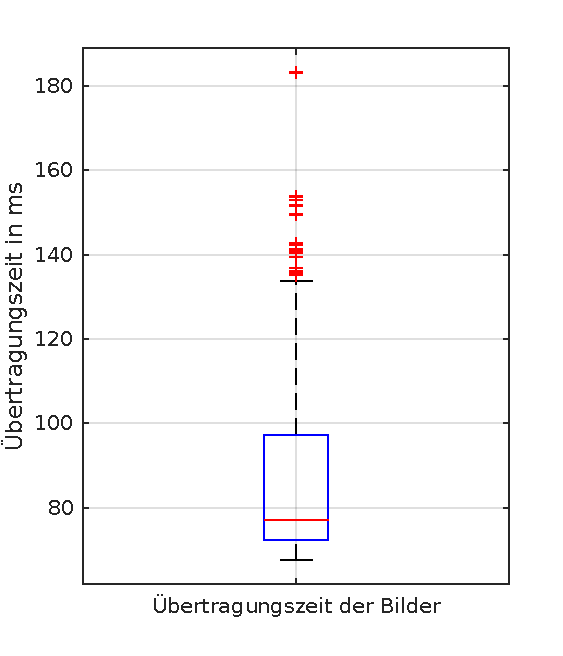
\includegraphics[width=0.7\textwidth]{evaluation_riverflow_times_pictransfer_3Hz_0_2m_s_boxplot}
	\label{fig:evaluation:riverflow:times_pictransfer_3Hz_0_2m_s_boxplot}
	\caption{Übertragungszeit der Aufnahmen bei \SI{3}{\hertz} Bildfrequenz}
\end{figure}

\section{Geschwindigkeit \dcfirstauthorshort}
\label{ssec:evaluation:messungen:geschwindigkeit}
%In diesem Abschnitt soll untersucht werden, ob eine Reduzierung der Geschwindigkeit positive Auswirkungen auf die Zuverlässigkeit von Bildverarbeitung und Regelung besitzt.

Nachdem eine passende Einstellung der Regel-und Bildverarbeitungsfrequenz gefunden wurde, soll nun das Fahren mit höheren Geschwindigkeiten betrachtet werden. Neben der Sichtprüfung der Funktionalität der Fahrspurverfolgung wurden die Anzahl der zur Zielpunktbestimmung genutzten Punkte pro Regelungsiteration und der prozentuale Anteil an nicht bestimmten Zielpunkten zur Untersuchung herangezogen. 

Zur besseren Vergleichbarkeit der Messergebnisse wurden die Daten für je eine entgegen des Uhrzeigersinnes gefahrene Runde mit \SI{3}{\hertz} Bildverarbeitungsfrequenz aufgenommen.

Abbildung~\ref{fig:evaluation:riverflow:regelungspunkte:je_linie} zeigt exemplarisch für die Geschwindigkeit \( \gls{lat:velocity} = 
\SI{0,2}{\metre\per\second} \) die  Anzahl jeweiliger Linienpunkttypen zur Zielpunktberechnung. Es fällt sogleich auf, dass die Mittellinie einen kleineren Einfluss nimmt. Da pro Strich und Bild nur ein Punkt in der Weltkarte 
eingetragen wird, ist deren Punkteanzahl geringer. Wie unter 
\ref{item:regelung:zielpunkt:holen:regeln:xcoord} in Kapitel 
\ref{ssec:regelung:zielpunkt:holen} beschrieben, werden die Regelungspunkte unter anderem nach ihrer x-Koordinate ausgewählt. In einer Linkskurve fallen dadurch mehr Punkte der linken Randlinie in das Suchfenster. Da die Strecke in 
der befahrenen Richtung vorrangig Linkskurven aufweist, werden im Mittel mehr linke als rechte Randpunkte zur Zielpunktberechnung herangezogen.

\begin{figure}[htbp] % [htb]
	\centering
	\subfloat[Anzahl der jeweiligen zur Regelung genutzten Punkte aus der Weltkarte bei \( \gls{lat:velocity} = \SI{0,2}{\metre\per\second} \) 
	\label{fig:evaluation:riverflow:regelungspunkte:je_linie}]{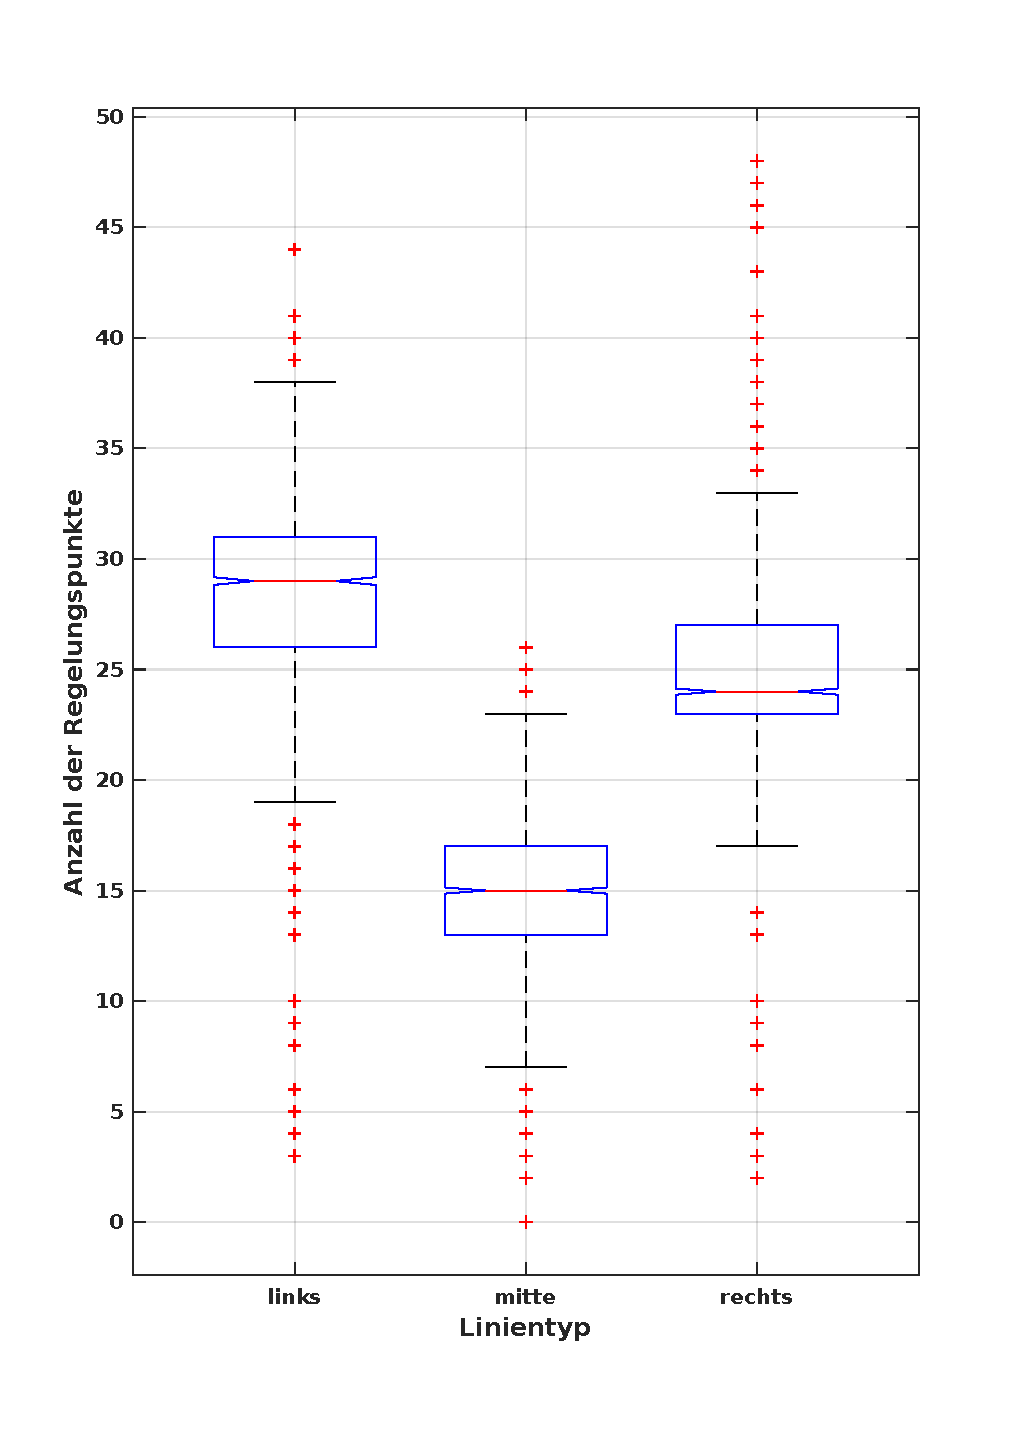
\includegraphics[height=0.35\textheight]{evaluation_riverflow_regelungspunkte_je_linie_0_2m_s_3Hz.pdf}}
	\hfill
	\subfloat[Anzahl der zur Regelung verwendeten Kartenpunkte zu verschiedenen 
	Geschwindigkeiten
	\label{fig:evaluation:riverflow:regelungspunkte:je_geschw}]{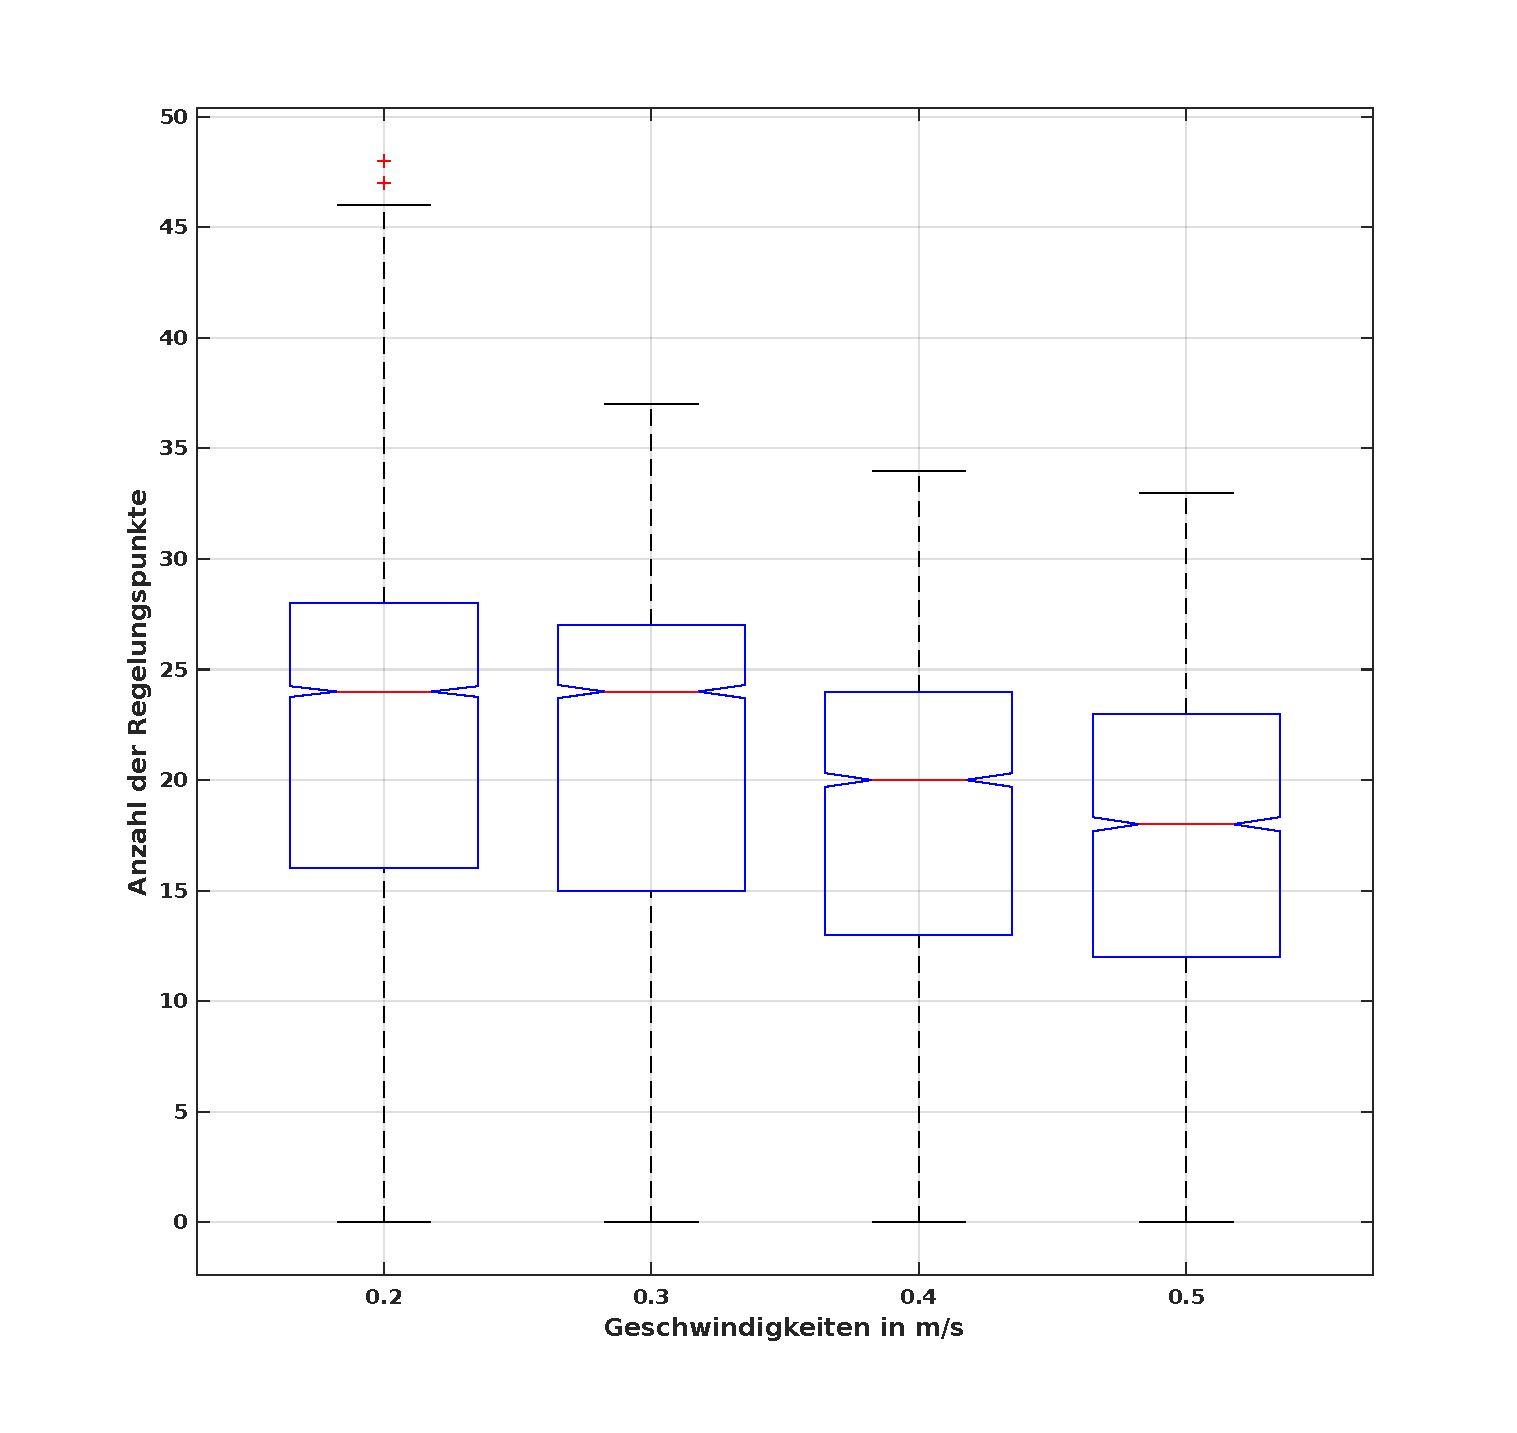
\includegraphics[height=0.35\textheight]{evaluation_riverflow_regelungspunkte_je_geschw_3Hz.pdf}}
	\caption{Boxplots zur Menge der Punkte, welche in einem Regelungsintervall 
	aus der Weltkarte entnommen und zur Zielpunktberechnung verwendet werden}
	\label{fig:evaluation:riverflow:regelungspunkte}
\end{figure}

Betrachten wir die Gesamtzahl der zur Regelung verwendeten Punkte, ist wie in 
Abbildung~\ref{fig:evaluation:riverflow:regelungspunkte:je_geschw} ein Abfallen der Anzahl mit ansteigender Geschwindigkeit des Fahrzeugs zu beobachten. Wenn das Auto schneller fährt, liegt ein Punkt in der Karte umso eher außerhalb des Bereiches, aus dem die Regelungspunkte genutzt werden. Bei gleichbleibender Bildfrequenz wird zwischen jedem Bild eine größere Strecke zurückgelegt, sodass die Dichte der Weltkartenpunkte geringer wird. Der dargestellte Boxplot erfüllt also die Erwartungen.

Die mit unserer Implementierung erreichbare Höchstgeschwindigkeit sollte folglich dann erreicht sein, wenn der mobile Roboter fast ausschließlich nach den Informationen eines Bildes regelt oder sogar zwischenzeitlich keine Zielpunkte mangels Regelungspunkten bestimmen kann. Mit anderen Worten: Wenn sich das Auto zwischen zwei Aufnahmen bis zum Sichtende des ersten Bildes bewegt, wie der Riverflow-Algorithmus Punkte erkennen konnte, ist die Maximalgeschwindigkeit beinahe erreicht. Ein Indiz dafür ist neben der visuellen Auffälligkeit des Fahrspurverlasses die starke Zunahme der nicht gefundenen Zielpunkte. 

\begin{figure}[htbp] % [htb]
	\centering
	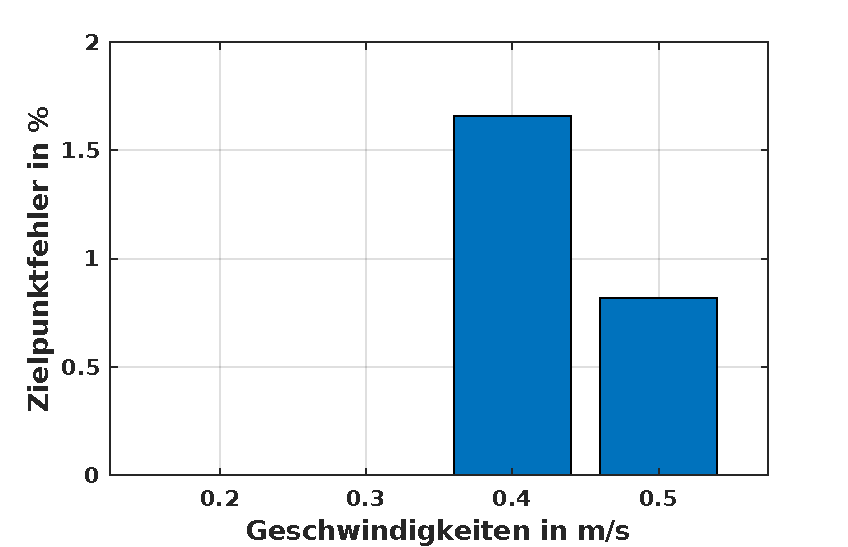
\includegraphics[width=0.7\textwidth]{evaluation_riverflow_zielpunktfehler_je_geschw_3Hz.pdf}
	\caption{Anteil der unbestimmten Zielpunkte einer Runde auf dem Parcours mit verschiedenen Geschwindigkeiten}
	\label{fig:evaluation:riverflow:zielpunktfehler_je_geschw}
\end{figure}

Was in Abbildung~\ref{fig:evaluation:riverflow:zielpunktfehler_je_geschw} zu sehen ist, war ebenfalls während des Fahrversuches am Auto zu beobachten. Ab einer Geschwindigkeit von \( \gls{lat:velocity} = \SI{0,4}{\metre\per\second} \) fuhr das Fahrzeug instabiler und die Latenzzeit der Regelung war dahingehend zu bemerken, dass in Kurven meist etwas zu spät und kurz darauf zur Korrektur zu viel eingelenkt wurde. Dies führte zu einer schwingenden Fahrweise (das Auto fuhr \glqq Schlängellinien\grqq). 

Die begrenzende Komponente für die Geschwindigkeit ist hier neben der Bildfrequenz allerdings auch das Getriebe. Durch dessen kurze Übersetzung beträgt die Geschwindigkeit im Maximum 4500 tics pro Sekunde, was in etwa \SI{0,43}{\metre\per\second} entspricht. Die im Plot bezeichneten \SI{0,5}{\metre\per\second} dürften folglich nicht genau stimmen, auch wenn dies der eingestellte Wert des Geschwindigkeitsparameters war. Sie geben die Daten zu der dem ersten Auto maximal physikalisch möglichen Geschwindigkeit an. 

Ergänzend muss hier erwähnt werden, dass bereits ein zweites Fahrzeug mit ca. doppelt so langer Übersetzung existiert. Jedoch misslang eine Testfahrt mit unveränderten Parametereinstellungen bei höheren Geschwindigkeiten. Auch hier zeigte sich die Grenze an der \SI{0,5}{\metre\per\second}-Marke.

Dass diese Geschwindigkeit auch die Grenze der Stabilität des Algorithmus war, zeigte ein \glqq Dauertest\grqq{} von zehn Runden. Bis zu einer Geschwindigkeit von \SI{0,3}{\metre\per\second} führte der Versuch zu keinen nennenswerten Problemen in der Fahrspurverfolgung. Auch wenn während der schnelleren \SI{0,4}{\metre\per\second}-Fahrt zehn Runden erfolgreich abgefahren wurden, kam hier das Fahrzeug mitunter stark ins Schwingen und befand sich kurz davor, den Fahrstreifen zu verlieren. Mit der höchstmöglichen Geschwindigkeit wurde der Dauertest nicht bestanden, da das Auto schon nach zwei Runden von der Straße abkam.

\subsubsection{Leistungsfähigkeit bei Veränderung der Umgebungsbedingungen - Störobjekte}
Da geplant ist die Teststrecke in Zukunft realistischer zu gestalten, d.h. Objekte wie Straßenschilder, andere Fahrzeuge, Personen und Gebäude hinzuzufügen. Der Einfluss solcher \glqq Störobjekte\grqq\ auf den Fahrspurverfolgungsalgorithmus soll nun untersucht werden.

\paragraph{Menge der Objekte in einem Bild}
Zu Beginn soll lediglich die Menge der \glqq Störobjekte\grqq\, welche sich in einem Bild befinden, variiert werden. Da sich die Objekte hinreichend weit von der Fahrbahnmarkierung entfernt befinden, ist kein Einfluss die Bildverarbeitung zu erwarten.

\paragraph{Entfernung der Objekte von den Fahrbahnmarkierungen}
Verringert man die Distanz zwischen \glqq Störobjekten\grqq\ und der Straße, wird es wahrscheinlicher, dass Kanten dieser Gegenstände als Fahrbahnmarkierung erkannt werden.

\paragraph{Kontrast der Objekte im Vergleich zum Testszenario}
Ist der Helligkeitsunterschied zwischen Fahrbahn und \glqq Störobjekt\grqq\ bzw. der leeren Fläche neben der Fahrbahn und dem \glqq Störobjekt\grqq\ sehr gering, so sollte keine zusätzliche Kante im Bild gefunden und als Fahrbahnmarkierung identifiziert werden . Diese These soll im folgenden Test bestätigt betrachtet werden.

\subsubsection{Leistungsfähigkeit bei Veränderung der Umgebungsbedingungen - fehlende Fahrbahnmarkierungen}
Es soll gezeigt werden, dass auch bei fehlen bestimmter Fahrbahnmarkierungen eine Verfolgung des Straßenverlaufs möglich ist.






